\documentclass[aspectratio=169,10pt]{beamer}

\usetheme{Madrid}
\usecolortheme{seahorse}
\useinnertheme{rectangles}
\useoutertheme{infolines}
\setbeamertemplate{navigation symbols}{}
\setbeamercolor{frametitle}{bg=structure.fg!85!black,fg=white}
\setbeamercolor{title}{bg=structure.fg!85!black,fg=white}

\usepackage{amsmath,amssymb}
\usepackage{booktabs}
\usepackage{array}
\usepackage{tikz}
\usetikzlibrary{arrows.meta,positioning,calc,shapes.geometric,backgrounds,fit}
\usepackage{pgfplots}
\pgfplotsset{compat=1.18}

\title[EADD for MLOps Feature Monitoring]{Enhanced Adversarial Drift Detection \\ for MLOps Feature Monitoring}
\author[Begum et al.]{Nusrat Begum\inst{1} \and Phaphontee Yamchote\inst{1} \and \\ Chainarong Amornbunchornvej\inst{2} \and Thanapon Noraset\inst{1}}
\institute[Mahidol \& NECTEC]{\inst{1}Faculty of ICT, Mahidol University \\ \inst{2}NECTEC, NSTDA, Thailand}
\date{JCSSE 2026 \\ Bangkok, June 24--27, 2026}

\begin{document}

% ─────────────────────────────────────────────
\begin{frame}
\titlepage
\end{frame}

% ─────────────────────────────────────────────
\begin{frame}{Outline}
\begin{columns}[T]
\column{0.5\textwidth}
\begin{enumerate}
  \item Motivation \& Problem
  \item Background: C2ST \& D3
  \item EADD Pipeline
  \item ASPT (Contribution~1)
  \item SHAP + DSI (Contribution~2)
\end{enumerate}
\column{0.5\textwidth}
\begin{enumerate}\setcounter{enumi}{5}
  \item Experimental Setup
  \item Results
  \item Ablation \& Runtime
  \item Limitations \& Future Work
  \item Conclusion
\end{enumerate}
\end{columns}
\end{frame}

% ═══════════════════ MOTIVATION ═══════════════════
\begin{frame}{Motivation: Production ML Models Fail Silently}
\begin{columns}[T]
\column{0.55\textwidth}
\textbf{Distribution drift} degrades models in production.

\medskip

\textbf{Existing detectors answer only one question:}
\begin{itemize}
  \item \textcolor{red}{\textbf{Whether}} drift occurred (binary alarm)
\end{itemize}

\medskip

\textbf{Practitioners need to know:}
\begin{itemize}
  \item \textcolor{blue}{\textit{Which}} features drifted?
  \item \textcolor{blue}{\textit{How severe}} is the shift?
  \item \textcolor{blue}{\textit{Is it real}} or autocorrelation noise?
\end{itemize}

\column{0.45\textwidth}
\begin{block}{D3 [Gözüaçık et al., CIKM 2019]}
Most robust unsupervised detector (Lukats et al., 2024). \\[2pt]
But has \textbf{3 gaps}:
\begin{itemize}\small
  \item No formal significance test
  \item No feature attribution
  \item Linear classifier (misses non-linear drift)
\end{itemize}
\end{block}
\end{columns}
\end{frame}

% ─────────────────────────────────────────────
\begin{frame}{Research Gap}
\centering
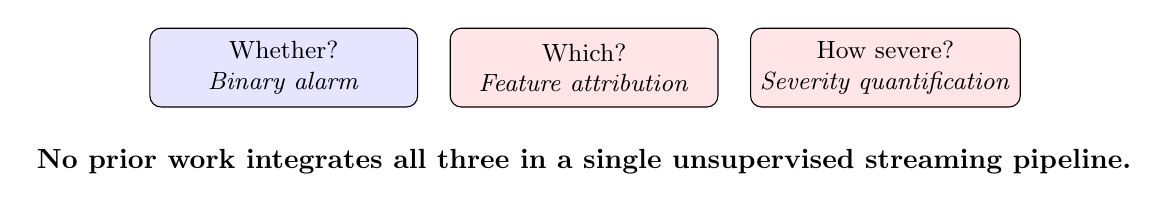
\begin{tikzpicture}[node distance=4mm, font=\small]
\node[draw, rounded corners, fill=blue!10, minimum width=3.4cm, minimum height=1cm, align=center] (whether) {Whether? \\ \textit{Binary alarm}};
\node[draw, rounded corners, fill=red!10, right=of whether, minimum width=3.4cm, minimum height=1cm, align=center] (which) {Which? \\ \textit{Feature attribution}};
\node[draw, rounded corners, fill=red!10, right=of which, minimum width=3.4cm, minimum height=1cm, align=center] (severe) {How severe? \\ \textit{Severity quantification}};
\node[below=0.4cm of which, font=\bfseries] {No prior work integrates all three in a single unsupervised streaming pipeline.};
\end{tikzpicture}

\bigskip

\textbf{This paper:} Enhanced Adversarial Drift Detection (EADD)\\
$\Rightarrow$ \textit{whether}, \textit{when}, \textit{which}, \textit{how severe} in one pipeline.
\end{frame}

% ═══════════════════ CONTRIBUTIONS ═══════════════════
\begin{frame}{Three Contributions}
\begin{enumerate}\setlength\itemsep{0.6em}
\item \textbf{Adaptive Sequential Permutation Test (ASPT)} \\
      Gates drift via formal permutation test; \textbf{90--95\% fewer} permutations vs.\ fixed budget; preserves Type~I error.
\item \textbf{SHAP-Based Localisation + Drift Severity Index (DSI)} \\
      $\mathrm{DSI} = \mathrm{AUC} \times (1 - H_{\mathrm{norm}}(\mathbf{s}))$ \\
      Identifies \textit{which} features drifted; quantifies \textit{how severe}.
\item \textbf{Comprehensive Benchmark} \\
      EADD vs.\ 7 unsupervised detectors on synthetic + 13 real-world streams.
\end{enumerate}
\end{frame}

% ═══════════════════ PIPELINE ═══════════════════
\begin{frame}{EADD Pipeline}
\centering
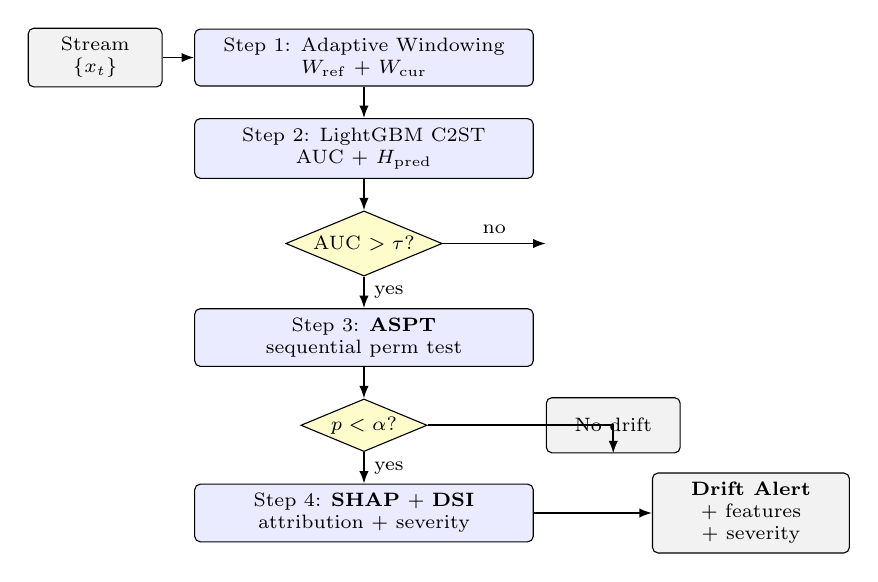
\begin{tikzpicture}[
    font=\scriptsize, node distance=4mm,
    box/.style={draw, rounded corners=2pt, fill=blue!8, minimum width=4.3cm, minimum height=0.7cm, align=center},
    dec/.style={diamond, draw, fill=yellow!20, aspect=2.4, align=center, inner sep=1pt},
    term/.style={draw, rounded corners=2pt, fill=gray!10, align=center, minimum width=1.7cm, minimum height=0.7cm},
    arr/.style={-{Latex[length=1.6mm]}, semithick},
]
\node[term] (in) {Stream\\$\{x_t\}$};
\node[box, right=of in] (s1) {Step 1: Adaptive Windowing\\$W_{\mathrm{ref}}$ + $W_{\mathrm{cur}}$};
\node[box, below=of s1] (s2) {Step 2: LightGBM C2ST\\AUC + $H_{\mathrm{pred}}$};
\node[dec, below=of s2] (d1) {AUC $> \tau$?};
\node[box, below=of d1] (s3) {Step 3: \textbf{ASPT}\\sequential perm test};
\node[dec, below=of s3] (d2) {$p < \alpha$?};
\node[box, below=of d2] (s4) {Step 4: \textbf{SHAP} + \textbf{DSI}\\attribution + severity};
\node[term, right=1.5cm of d2] (nodrift) {No drift};
\node[term, right=1.5cm of s4, minimum width=2.5cm] (alert) {\textbf{Drift Alert}\\+ features\\+ severity};

\draw[arr] (in) -- (s1);
\draw[arr] (s1) -- (s2);
\draw[arr] (s2) -- (d1);
\draw[arr] (d1) -- node[right,font=\scriptsize]{yes} (s3);
\draw[arr] (s3) -- (d2);
\draw[arr] (d2) -- node[right,font=\scriptsize]{yes} (s4);
\draw[arr] (d1.east) -- node[above,font=\scriptsize]{no} (d1.east -| nodrift.west);
\draw[arr] (d2.east) -| (nodrift.south);
\draw[arr] (s4) -- (alert);
\end{tikzpicture}
\end{frame}

% ═══════════════════ ASPT ═══════════════════
\begin{frame}{Contribution 1: ASPT}
\textbf{Problem:} D3 uses fixed AUC threshold $\to$ false alarms on autocorrelated data.

\textbf{Solution:} permutation test with adaptive early stopping.

\begin{block}{ASPT decision rule (per permutation $i$)}
\begin{itemize}\small
  \item \textbf{Early reject} $H_0$: if $c_i{=}0$, $i{\ge}B_{\min}$, $1/(i{+}1)<\alpha$ \\
        $\to$ confirm drift with $p = 1/(i{+}1)$
  \item \textbf{Early accept} $H_0$: if $c_i/i > 2\alpha$, $i{\ge}B_{\min}$ \\
        $\to$ no drift with $p = (c_i{+}1)/(i{+}1)$
  \item \textbf{Terminal:} $p = (c_{B_{\max}}{+}1)/(B_{\max}{+}1)$
\end{itemize}
\end{block}

\textbf{Result:} Drift terminates at $i{=}20$, stable at $i{=}10$, vs.\ $B_{\max}{=}199$ \\
$\Rightarrow$ \textbf{90--95\% permutation savings} while preserving overall $\alpha$.
\end{frame}

% ═══════════════════ SHAP + DSI ═══════════════════
\begin{frame}{Contribution 2: SHAP Attribution + DSI}
\begin{columns}[T]
\column{0.55\textwidth}
\textbf{SHAP on the discriminative classifier} \\
TreeSHAP on the LightGBM gate (which D3 discards):
\[
\bar\phi_j = \tfrac{1}{n}\sum_i |\phi_j^{(i)}|, \quad
s_j = \bar\phi_j / \textstyle\sum_k \bar\phi_k
\]
$\Rightarrow$ ranks features by drift contribution.

\medskip
\textbf{Drift Severity Index (DSI):}
\[
\mathrm{DSI} = \mathrm{AUC} \times \bigl(1 - H_{\mathrm{norm}}(\mathbf{s})\bigr)
\]
$H_{\mathrm{norm}} \in [0,1]$ via $\log_2 d$ normalisation $\to$ dimensionality-invariant.

\column{0.45\textwidth}
\begin{block}{DSI prescription tiers}
\small
\begin{tabular}{ll}
\toprule
\textbf{DSI} & \textbf{Action} \\
\midrule
$>0.6$ & Critical: audit pipeline \\
$0.3$--$0.6$ & Moderate: shared source \\
$<0.3$ & Low: scheduled retrain \\
\bottomrule
\end{tabular}
\\[3pt]
{\scriptsize (Heuristic tiers; require domain calibration.)}
\end{block}
\end{columns}
\end{frame}

% ═══════════════════ EXPERIMENTS ═══════════════════
\begin{frame}{Experimental Setup}
\textbf{Synthetic} ($n{=}5{,}000$, $d{=}5$): four drift patterns + four stable streams.

\textbf{Real-world} (13 streams): 4 annotated INSECTS + 9 unannotated.

\textbf{SHAP attribution} ($n{=}10{,}000$, $d{=}10$, drift at $t{=}5{,}000$): univariate / subset / multivariate.

\textbf{Baselines:} D3, BNDM, CSDDM, IBDD, OCDD, SPLL, UDetect (Lukats et al.\ 2024).

\medskip
\textbf{Configuration:} LightGBM (50 trees), $N_{\mathrm{ref}}{=}500$, $N_{\mathrm{cur}}{=}200$, $M{=}50$, \\ ASPT $B_{\max}{=}199$, $B_{\min}{=}10$, $\alpha{=}0.05$, $\tau{=}0.7$.
\end{frame}

% ─────────────────────────────────────────────
\begin{frame}{Result 1: Synthetic Coverage + False Alarms}
\centering\small
\begin{tabular}{lcccc}
\toprule
\textbf{Detector} & \textbf{Types} & \textbf{Coverage} & \textbf{Mean FA} & \textbf{Lift} \\
\midrule
\textbf{EADD}  & \textbf{4/4} & \textbf{100\%} & \textbf{0.00} & \textbf{1.00} \\
BNDM   & 4/4 & 100\% & 4.75  & 5.75 \\
CSDDM  & 4/4 & 100\% & 5.50  & 6.50 \\
IBDD   & 4/4 & 100\% & 46.25 & 47.25 \\
OCDD   & 4/4 & 100\% & 17.50 & 18.50 \\
D3     & 2/4 & 50\%  & 0.00  & 1.00 \\
SPLL   & 2/4 & 50\%  & 0.00  & 1.00 \\
UDetect& 0/4 & 0\%   & n/a   & n/a  \\
\bottomrule
\end{tabular}

\bigskip
\textbf{EADD: only detector with full coverage AND zero false alarms.}
\end{frame}

% ─────────────────────────────────────────────
\begin{frame}{Result 2: Real-World INSECTS — Faster Detection}
\centering\small
\begin{tabular}{lcccc}
\toprule
\textbf{Dataset} & \textbf{Prec.} & \textbf{Recall} & \textbf{MTD (EADD)} & \textbf{MTD (D3)} \\
\midrule
InsectsAbrupt      & 0.33 & 0.60 & \textbf{135} & 155.5 \\
InsectsGradual     & n/a  & 0/1  & n/a          & n/a   \\
InsectsIncrAbrupt  & 0.14 & 1.00 & \textbf{33}  & 272.5 \\
InsectsIncrRecur   & 0.17 & 1.00 & \textbf{133} & 323.5 \\
\bottomrule
\end{tabular}

\bigskip
\begin{itemize}
\item EADD beats D3 on MTD in all three jointly detected cases.
\item \textbf{Up to 8$\times$ faster} on incremental drift (33 vs.\ 272.5).
\end{itemize}
\end{frame}

% ─────────────────────────────────────────────
\begin{frame}{Result 3: SHAP Attribution Accuracy}
\centering\small
\begin{tabular}{lccccc}
\toprule
\textbf{Scenario} & \textbf{AUC} & \textbf{P@k} & \textbf{R@k} & \textbf{Top feature (\%)} & \textbf{DSI} \\
\midrule
Univariate (1/10)   & 0.784 & 1.0 & 1.0 & F3 (52.3\%) & 0.193 \\
Subset (3/10)       & 0.809 & 1.0 & 1.0 & F5 (24.5\%) & 0.096 \\
Multivariate (10/10)& 0.806 & 1.0 & 1.0 & F2 (14.6\%) & 0.016 \\
\bottomrule
\end{tabular}

\bigskip
\begin{itemize}
\item Perfect attribution: \textbf{P@k = R@k = 1.0} for all 3 scenarios.
\item Meaningful result: \textbf{univariate} (1/10 features correctly ranked first).
\item DSI orders by concentration: univariate $>$ subset $>$ multivariate.
\end{itemize}
\end{frame}

% ─────────────────────────────────────────────
\begin{frame}{Result 4: False Alarm Robustness}
\centering\small
\begin{tabular}{lccc}
\toprule
\textbf{Stable stream} & \textbf{EADD} & \textbf{D3 ($\tau{=}0.6$)} & \textbf{D3 ($\tau{=}0.7$)} \\
\midrule
Gaussian i.i.d.       & 0 & 0    & 0    \\
Autocorrelated AR(1)  & \textbf{0} & 87.4 & 54.6 \\
Heteroscedastic       & 0 & 10.4 & 0    \\
Correlated $\rho{=}0.7$ & 0 & 10.0 & 0    \\
\bottomrule
\end{tabular}

\bigskip
\begin{itemize}
\item EADD: \textbf{0 false alarms} on all 4 stable types.
\item D3 vulnerable to autocorrelation (54.6 FA at $\tau{=}0.7$).
\item Mann--Whitney U: significant at $\tau{=}0.6$ ($p{=}0.0101$).
\end{itemize}
\end{frame}

% ─────────────────────────────────────────────
\begin{frame}{Ablation: Where Does the Gain Come From?}
\centering\small
\begin{tabular}{lcccc}
\toprule
\textbf{Variant} & \textbf{$d{=}10$} & \textbf{$d{=}20$} & \textbf{$d{=}50$} & \textbf{Coverage} \\
\midrule
EADD-Full              & 6.93s  & 10.76s & 23.11s & 4/4 \\
EADD$_{-\mathrm{ASPT}}$ & 6.68s  & 10.43s & 22.64s & 4/4 \\
D3                     & 0.07s  & 0.09s  & 0.14s  & 2/4 \\
\bottomrule
\end{tabular}

\medskip
\textbf{EADD-Full vs.\ EADD$_{-\mathrm{ASPT}}$ differ by $<\!5\%$:}
\begin{itemize}
\item \textbf{Coverage gain} (4/4 vs.\ D3's 2/4) $\Rightarrow$ \textbf{LightGBM upgrade}.
\item \textbf{ASPT role} $\Rightarrow$ significance control on autocorrelated streams \\
      (suppresses 54.6 spurious detections at $\tau{=}0.7$).
\item ASPT's 90--95\% saving is \textit{within} the significance stage, \\
      orthogonal to LightGBM-driven $\sim$80--160$\times$ overhead vs.\ D3.
\end{itemize}
\end{frame}

% ─────────────────────────────────────────────
\begin{frame}{Limitations \& Future Work}
\textbf{Limitations}
\begin{itemize}\small
\item Wall-clock $\sim$50--160$\times$ D3 — dominated by LightGBM training every $M{=}50$ steps.
\item \textbf{Multiple testing over time:} $\sim$600 tests over 30K samples; Bonferroni $\alpha'{\approx}8.3{\times}10^{-5}$ below ASPT's $1/(B_{\max}{+}1){=}0.005$ floor. Zero-FA result is empirical, not theoretically guaranteed.
\item DSI tier boundaries are heuristics, never triggered (all DSI $<0.3$ in experiments).
\item SHAP attributions are correlational, not causal.
\item No isolation of reservoir sampling vs.\ window config contributions.
\end{itemize}

\medskip
\textbf{Future Work}
\begin{itemize}\small
\item Anytime-valid e-values for streaming FWER control.
\item Causal attribution methods (Budhathoki et al.).
\item Multi-domain DSI calibration to ground tier boundaries.
\item Adversarial robustness of discriminative detectors.
\end{itemize}
\end{frame}

% ═══════════════════ CONCLUSION ═══════════════════
\begin{frame}{Conclusion}
\textbf{EADD extends discriminative drift detection with:}
\begin{enumerate}
\item ASPT $+$ $H_{\mathrm{pred}}$: rigorous confirmation, 90--95\% perm savings.
\item SHAP $+$ DSI: feature-level diagnosis $+$ severity quantification.
\item Benchmark vs.\ 7 unsupervised detectors on synthetic $+$ real-world.
\end{enumerate}

\medskip
\textbf{Headline results:}
\begin{itemize}
\item \textbf{4/4} synthetic coverage with \textbf{0} false alarms (only detector to achieve both).
\item Up to \textbf{8$\times$} faster MTD than D3 on incremental INSECTS streams.
\item \textbf{P@k = R@k = 1.0} on univariate SHAP attribution.
\item \textbf{0} false alarms vs.\ D3's \textbf{54.6} on autocorrelated streams ($p{=}0.0101$).
\end{itemize}

\medskip
\centering
\textit{EADD answers \textbf{whether}, \textbf{when}, \textbf{which}, \textbf{how severe} in one pipeline.}
\end{frame}

% ─────────────────────────────────────────────
\begin{frame}[plain]
\vspace*{\fill}
\centering
{\Huge Thank you.}\\[1em]
{\Large Questions?}\\[2em]
{\small
Nusrat Begum --- \texttt{nusrat.beg@student.mahidol.ac.th}\\[0.4em]
Code + paper available at the project repository.
}
\vspace*{\fill}
\end{frame}

% ─────────────────────────────────────────────
\appendix
\begin{frame}{Backup: Runtime Scaling — Window $N_{\mathrm{cur}}$}
\centering\small
\begin{tabular}{lcccc}
\toprule
\textbf{Variant} & \textbf{$N{=}100$} & \textbf{$N{=}200$} & \textbf{$N{=}500$} & \textbf{$N{=}1000$} \\
\midrule
EADD-Full            & 5.83s & 6.91s & 10.52s & 11.22s \\
EADD$_{-\mathrm{ASPT}}$ & 5.62s & 6.68s & 10.23s & 10.58s \\
D3                   & 0.11s & 0.07s & 0.04s  & 0.03s  \\
\bottomrule
\end{tabular}

\bigskip
\begin{itemize}
\item $N_{\mathrm{cur}}{=}200{\to}1000$: EADD time grows only \textbf{1.6$\times$}.
\item LightGBM cost sub-linear in $N$, near-linear in $d$.
\end{itemize}
\end{frame}

\begin{frame}{Backup: Correlated Features ($d{=}10$)}
\centering\small
\begin{tabular}{lcc}
\toprule
\textbf{Correlation $\rho$} & \textbf{EADD first-detect} & \textbf{D3 first-detect} \\
\midrule
$0.0$ & $t{=}4099$ & $t{=}4117$ \\
$0.5$ & $t{=}4099$ & $t{=}4117$ \\
$0.9$ & $t{=}4099$ & $t{=}4117$ \\
\bottomrule
\end{tabular}

\bigskip
\begin{itemize}
\item Cholesky-mixed Gaussian; $+2\sigma$ shift in 3 features at $t{=}4000$.
\item EADD detection robust to correlation; stable correlated streams give 0 FA.
\item SHAP under correlation $\to$ interpret at feature-group granularity.
\end{itemize}
\end{frame}

\end{document}
